\documentclass[%
%reprint,
%superscriptaddress,
%groupedaddress,
%unsortedaddress,
%runinaddress,
%frontmatterverbose, 
% preprint,
%preprintnumbers,
 nofootinbib,
%nobibnotes,
%bibnotes,
 amsmath,amssymb,
 aps,
%pra,
%prb,
%rmp,
%prstab,
%prstper,
%floatfix,
 twocolumn,
 superscriptaddress
]{revtex4-2}


\usepackage{aas_macros}
\usepackage{amssymb}
\usepackage{amsmath}
\usepackage{array}
\usepackage{color,units}
\usepackage[dvipsnames]{xcolor} % for more colours!
\usepackage{lineno}
\usepackage{dcolumn}
\usepackage{longtable}
\usepackage[normalem]{ulem} %% for striking out text
\usepackage{subfigure}
\usepackage[T1]{fontenc}
\usepackage[breaklinks]{hyperref}
\usepackage{booktabs}
\usepackage{xspace} 
\usepackage{bm}% bold math
\usepackage{graphicx} % Include figure files
% \usepackage{authblk}

\graphicspath{{images/}} %Setting the graphicspath

% symbols
\DeclareSymbolFont{extraup}{U}{zavm}{m}{n}
\DeclareMathSymbol{\varheart}{\mathalpha}{extraup}{86}
\DeclareMathSymbol{\vardiamond}{\mathalpha}{extraup}{87}


% Keywords
\newcommand{\bilby}{{\sc \href{https://lscsoft.docs.ligo.org/bilby/}{\texttt{Bilby}}}\xspace}
\newcommand{\bilbypipe}{{\sc \texttt{bilby\_pipe}}\xspace}
\newcommand{\dynesty}{{\sc \texttt{dynesty}}\xspace}
\newcommand{\cpnest}{{\sc cpnest}\xspace}
\newcommand{\ptemcee}{{\sc ptemcee}\xspace}
\newcommand{\gwpy}{{\sc \href{https://gwpy.github.io/}{\texttt{GWpy}}}\xspace}
\newcommand{\imrphenomp}{{\sc IMRPhenomPv2}\xspace}
\newcommand{\seob}{{\sc SEOBNRv4PHM}\xspace}


\newcommand{\gstlal}{{\sc GstLAL}\xspace}
\newcommand{\cwb}{{\sc cWB}\xspace}
\newcommand{\spiir}{{\sc SPIIR}\xspace}
\newcommand{\mbta}{{\sc MBTAOnline}\xspace}
\newcommand{\pycbc}{{\sc \href{https://pycbc.org/}{{PyCBC}}}\xspace}

\newcommand{\GWTC}{{\sc \href{https://ui.adsabs.harvard.edu/abs/2019PhRvX...9c1040A/abstract}{{GWTC-1}}}\xspace}
\newcommand{\OGC}{{\sc \href{https://ui.adsabs.harvard.edu/abs/2020ApJ...891..123N/abstract}{{2-OGC}}}\xspace}
\newcommand{\IAS}{{\sc \href{https://ui.adsabs.harvard.edu/abs/2020PhRvD.101h3030V/abstract}{{IAS}}}\xspace}


% math keywords 
\newcommand{\fancytext}[1]{{\relax\ifmmode#1\else $#1$\fi}\xspace}
\newcommand{\mathcmd}[1]{{\sc \relax\ifmmode#1\else $#1$\fi}\xspace}
\newcommand{\bcr}{\mathcmd{\rho_\text{BCR}}}
\newcommand{\pycbcstat}{\mathcmd{\rho_\text{PC}}}
\newcommand{\snr}{\mathcmd{\rho}}
\newcommand{\psd}{\mathcmd{P(f)}}
\newcommand{\msun}{\mathcmd{\text{M}_\odot}}
\newcommand{\mtot}{\mathcmd{M}}
\newcommand{\parameters}{\mathcmd{\vec{\theta}}}
\newcommand{\prior}{\mathcmd{\pi(\parameters)}}
\newcommand{\template}{\mathcmd{\mu(\parameters)}}
\newcommand{\fap}{\mathcmd{\text{FAP}}}

\newcommand{\pastro}{\fancytext{p_\text{astro}}}
\newcommand{\pastrobcr}{\fancytext{p_\text{astro}^{\text{BCR}}}}
\newcommand{\untunedpastrobcr}{\fancytext{p_\text{astro}^{\text{BCR}\prime}}}
\newcommand{\pastroext}{\fancytext{p_\text{astro}^{\text{ext}}}}
\newcommand{\pval}{\fancytext{\text{p-value}}}
% Table settings
\renewcommand{\aboverulesep}{0pt}
\renewcommand{\belowrulesep}{0pt}
% \setlength\cellspacetoplimit{2pt}
% \setlength\cellspacebottomlimit{2pt}

\newcolumntype{C}{>{\centering\arraybackslash}X}
\newcolumntype{L}{>{\arraybackslash}X}

% Aesthetic colours
\definecolor{dodgerblue}{HTML}{1E90FF}
\definecolor{viennared}{HTML}{DA0A14}
\definecolor{ctorange}{HTML}{FF6C0C}
\definecolor{wales}{HTML}{ff0038}
\definecolor{benettongreen}{HTML}{009421}
\definecolor{valenciacfred}{HTML}{ee3524}
\definecolor{barcelonafcgold}{HTML}{edbb00}
\definecolor{jam}{HTML}{A50B5E}
\definecolor{austriawien}{HTML}{441678}
\definecolor{italia90green}{HTML}{009966}
\definecolor{ferrarired}{HTML}{ff2800}
\definecolor{gray}{HTML}{F0F0F0}
\definecolor{LightCyan}{rgb}{0.88,1,1}
\newcolumntype{a}{>{\columncolor{gray}}c}
\newcolumntype{b}{>{\columncolor{white}}c}

% author comments
\newcommand{\avi}[1]{\textcolor{orange}{[AV: #1]}}
\newcommand{\greg}[1]{\textcolor{purple}{[Greg: #1]}}
\newcommand{\rs}[1]{\textcolor{red}{[RS: #1]}}
\newcommand{\et}[1]{\textcolor{blue}{[ET: #1]}}



\begin{document}


\title{A search for high-mass black holes in data from the second LIGO observing run using a Bayesian ranking-statistic}



%------ affiliation shortcuts
\newcommand{\SPAno}{1}
\newcommand{\OzGravMonashno}{2}
\newcommand{\CITno}{3}
\newcommand{\MITno}{4}
\newcommand{\Kavlino}{5}

%--------------------------
\newcommand{\SPA}{School of Physics and Astronomy, Monash University, Clayton VIC 3800, Australia}
\newcommand{\OzGravMonash}{OzGrav: The ARC Centre of Excellence for Gravitational Wave Discovery, Clayton VIC 3800, Australia}
\newcommand{\MIT}{LIGO Laboratory, Massachusetts Institute of Technology, Cambridge, MA 02139, USA}
\newcommand{\Kavli}{Department of Physics and Kavli Institute for Astrophysics and Space Research, Massachusetts Institute of Technology, \\ 77 Massachusetts Ave, Cambridge, MA 02139, USA}
\newcommand{\CIT}{LIGO Laboratory, California Institute of Technology, Pasadena, CA 91125, USA}
\author{
\parbox{\textwidth}{
A.~Vajpeyi$^{\SPAno,\OzGravMonashno}$, %ORCID:0000-0002-4146-1132
R.~Smith$^{\SPAno,\OzGravMonashno}$, %ORCID:0000-0001-8516-3324
E.~Thrane$^{\SPAno,\OzGravMonashno}$, %0000-0002-4418-3895
G.~Ashton$^{\SPAno,\OzGravMonashno}$, %ORCID:0000-0001-7288-2231 
J.~Kanner$^\CITno$, 
T.~Alford$^\CITno$, 
L.~Xiao$^\CITno$, %0000-0003-2703-449X
M.~Isi$^{\MITno,\Kavlino}$, %0000-0001-8040-9807
S.~Garza$^\CITno$, 
}\vspace{0.2cm}\\
$^1$\SPA\\
$^2$\OzGravMonash\\
$^3$\CIT\\
$^4$\MIT\\
$^5$\Kavli\\
}




\date{\today}


\begin{abstract}
The detection of an intermediate-mass black hole population ($10^2-10^6$~\msun) will provide probes to their formation environments (e.g., disks of active galactic nuclei, globular clusters) and illuminate a potential pathway to produce supermassive black holes. Numerous methods to search for $10^4-10^6\ \msun$ intermediate-mass black holes exist, while the primary method to find $10^2-10^3\ \msun$ is by identifying gravitational-waves emitted from the merger of stellar binaries. Ground-based gravitational-wave detectors are in principle sensitive to such mergers and have found one $142^{+28}_{-16}\ \msun$ intermediate-mass black hole. In reality, ground-based detectors are plagued with short-duration instrumental transients that mimic the gravitational-wave signals from mergers capable of producing intermediate-mass black holes, making their detection difficult. Here we demonstrate a ranking statistic utilizing Bayesian inference to detect high-mass binary black hole mergers (with a total mass $>55$~\msun). We apply this technique to the high-mass triggers during LIGO's second observing run to search for previously unresolved gravitational-wave signals from high-mass binary black holes. Our analysis does not discover new intermediate-mass black holes. However, we find support for some stellar mass binary black holes unreported in GWTC-1.
\end{abstract}


\maketitle

%%%%%%---SECTIONS---%%%%%%%%%%%%
\section{Introduction}
Since the 1970s, there has been a steady accumulation of evidence for stellar mass ($M_\text{BH} < 10^{2} \ \msun$) and supermassive black holes ($M_\text{BH} > 10^{6} \ \msun$)~\cite{Webster:1972:Natur, Balick:1974:ApJ, Ghez:1998:ApJ, Genzel:2010:RvMP, Abbott:2019:PhRvX, EventHorizonTelescopeCollaboration:2019:ApJL, Abbott:2020:arXiv}.  However, there is a deficiency of observational evidence for black holes in the `intermediate-mass' range $10^{2} - 10^{6}\ \msun$. The discovery of an intermediate-mass black hole population will bridge this observational gap, probe intermediate-mass formation environments (e.g. accretion disks of active galactic nuclei~\cite{Tagawa:2021:ApJ, Li:2021:arXiv, Samsing:2020:arXiv, Tagawa:2020:ApJ, Ishibashi:2020:A&A, Grobner:2020:A&A, Yang:2019:PhRvL, McKernan:2019:ApJL, Yang:2019:ApJ, McKernan:2018:ApJ, Bellovary:2016:ApJL, McKernan:2014:MNRAS, McKernan:2012:MNRAS}, the centers of dense stellar clusters~\cite{Banerjee:2021:MNRASa, Zevin:2021:ApJ,Mapelli:2021:arXiv,Weatherford:2021:ApJL, Bouffanais:2021:arXiv, Ballone:2021:MNRAS, Kumamoto:2021:arXiv, Banerjee:2021:MNRASb, Martinez:2020:ApJ, Romero-Shaw:2020:ApJL, Anagnostou:2020:PASA}, Population-III stars~\cite{Toubiana:2021:PhRvL, Farrell:2021:MNRAS, Safarzadeh:2020:ApJL, Liu:2020:MNRAS, Inayoshi:2017:MNRAS}), and illuminate our understanding of supermassive black hole formation~\cite{Askar:2021:MNRAS, ArcaSedda:2019:arXiv, Amaro-Seoane:2007:CQGra, Gurkan:2006:ApJL}. A variety of techniques have been employed to search for $10^{4} - 10^{6}\ \msun$ intermediate mass candidates (reverberation mapping~\cite{Peterson:2014:SSRv}, direct kinematic measurements~\cite{Schodel:2002:Natur, Kiziltan:2017:Natur}, applying macroscopic galaxy to black hole mass scaling relations ($M_{BH}$-$\sigma$ and $M_{BH}$-L relations)~\cite{Graham:2013:ApJ, Wevers:2017:MNRAS}, studying  X-ray luminosity and spectra~\cite{Greene:2004:ApJ, Lin:2020:ApJL}, gravitational lensing of light curves~\cite{paynter_evidence_2021}, and others~\cite{Greene:2020:ARA&A, Koliopanos:2017:mbhe, Mezcua:2017:IJMPD})). However, these observational techniques are challenging to use for intermediate mass black holes due to their small sphere of influence compared to super-massive black holes~\cite{Mezcua:2017:IJMPD}. Additionally, some candidates discovered with these techniques can be attributed to sources without intermediate-mass black holes (e.g. clusters of stellar-mass black holes~\cite{Ridolfi:2016:MNRAS, Freire:2017:MNRAS}, anisotropic emission from neutron stars~\cite{Israel:2017:MNRAS, RodriguezCastillo:2020:ApJ}), while others have high uncertainties due to the observational techniques utilized~\cite{Greene:2020:ARA&A}.

Compact binaries coalescences (CBCs) can provide unambiguous gravitational-wave signals for intermediate-mass candidates (e.g. the $142^{+28}_{-16}\ \msun$ remnant observed from the gravitational wave event GW190521~\cite{Abbott:2020:PhRvL}). Ground-based gravitational wave detectors can probe the lower-end $10^{2} - 10^{3}\ \msun$ of the intermediate mass range. 
 As a binary's total mass $\text{M}_{T}$ is associated with its gravitational-wave merger frequency, $f\sim \text{M}_{T}^{-1}$, systems with large $\text{M}_{T}$ have very low merger frequencies $f < 100\ \text{Hz}$. Hence, ground based gravitational wave detectors ($\sim 10^1 - 10^3\ \text{Hz}$) are sensitive to the last milliseconds of merging systems with $100 \msun < \text{M}_{T} < 400 \msun$~\cite{LIGOScientificCollaboration:2015:CQGra, Martynov:2016:PhRvD, Moore_2014}, while space-based detectors ($\sim 10^{-2} - 10^1\ \text{Hz}$) can study the full signals of merging systems with $10^4 \msun < \text{M}_{T} < 10^7 \msun$~\cite{ Moore_2014, Lu:2019:PhRvD}. 

Because of the short-duration of intermediate-mass gravitational-wave signals in ground-based detector data steams, handling data quality is critical to their detection. The low-frequency ranges of ground-based observatories are plagued with non-stationary terrestrial artifacts, called \textit{glitches}~\cite{ pycbc_short_duration_transients, pe_with_glitch, blip_glitches}. Some glitches, similar to signals from high total mass mergers, last for a fraction of a second, making them difficult to distinguish from the signals. These glitches that mimic astrophysical signals can severely decrease the confidence in detection of true gravitational-waves from high total mass mergers~\cite{pycbc_short_duration_transients}.

Although a significant fraction of the glitches can be removed by testing them for coherence amongst various ground based detectors and performing matched-filtering, these methods are insufficient to remove all the glitches~\cite{ pycbc_short_duration_transients, pe_with_glitch, blip_glitches}. One method to account for more glitches while searching for high total mass CBC gravitational-waves is by utilizing a Bayesian odds~\cite{bci, kanner2016leveraging, BCR1, BCR2, bcr_gw151216, bayesian_odds}. In this paper, we utilize a Bayesian method, called the Bayesian Coherence Odds-Ratio \bcr~\cite{BCR1}, to rank the candidate gravitational-wave signals from high-mass compact binary coalescences (systems with total masses in the range of $55-500\ \msun$) in the detector data recorded during O2. The \bcr used in this study is a bootstrap-Bayesian odds computed using Bayesian evidences that describe the explicit probability of data under the hypothesis that the data contains coherent signals vs incoherent glitches, and empirically calculated prior-odds that describe how likely each hypotheses is. \rs{Need to add another couple of sentences describing what is unique about this work. For instance, we study both foreground \textit{and} background events (which is the first time anyone's done a large-scale Bayesian analysis on background data). Suggest using this format: ``We highlight a number of innovations unique to this work. First...''} The high-mass candidate \bcr values are then used to calculate the probability that the candidate is of astrophysical origins, \pastrobcr. Finally, if the candidate has a \pastro reported by the the LIGO-Virgo-KAGRA (LVK) collaboration in \GWTC~\cite{GWTC1}, the \pycbc-team~\cite{pycbc_code, pycbc_og0, pycbc_og1, pycbc_og2, pycbc_og3, pycbc_og4, pycbc_og5, pycbc_og6, pycbc_single_det, pycbc_ogc_2}, by the Institute of Advanced study's team (\IAS)~\cite{IAS0, IAS1, IAS2}, or by \citet{bayesian_odds}, we compare their \pastro with the \pastrobcr.


We find that (a) high-mass events reported in the \GWTC, including GW170729 (the heaviest event in \GWTC) are very statistically significant $\pastrobcr>0.9$; (b) three out of the eight \IAS events and candidates have $\pastrobcr>0.5$, corroborating \IAS's detection claims for those events (GW170304, GW170727, GW170817A), and that (c) our ranking statistic does not identify any new intermediate-mass black holes, but does identify an unreported marginal stellar-mass binary black hole candidate, 170222 with $\pastrobcr\sim0.5$.

The remainder of this paper is structured as follows. We outline our methods, including details of our ranking statistic and the retrieval of our candidates in Section~\ref{sec:method}. We present details on the implementation of our analysis in Section~\ref{sec:Analysis}. Finally, we present our results in Section~\ref{sec:Results}, and discuss these results in the context of the significance of gravitational-wave candidates in Section~\ref{sec:Conclusion}.

\section{Method\label{sec:method}}

The standard framework to identify CBC gravitational-wave signals in data is by quantifying the significance of candidates with null-hypothesis significance testing~\cite{GWTC1, GWTC2}. In this framework, the candidates' ranking statistic is compared against a background distribution in a frequentist approach. The independent matched-filter searches, e.g. \pycbc~\cite{pycbc_og4}, \spiir~\cite{spiir} and \gstlal~\cite{sachdev2019gstlal}, and the coherent burst search \cwb~\cite{cwb} used by LVK to search for signals in gravitational-wave data all use ranking statistics in such a manner~\cite{GWTC1}. Both \pycbc and \gstlal's ranking statistic incorporate information of the relative likelihood that the data contains a coherent signal versus just noise. In contrast, \cwb's ranking statistic uses the information of coherent energy present in the network of detectors~\cite{GWTC1}. 

Bayesian inference offers an alternative means to rank the significance of candidate events by computing the odds that the data contain a transient gravitational-wave signal vs. instrumental glitches or noise~\cite{BCR1}. This method relies on accurate models for the signal and glitch morphologies and populations~\cite{BCR1}. In principle, Bayesian odds is the optimal method for hypothesis testing~\cite{BCR2}. Much of its power comes from the Bayesian ``evidence'': a marginalized likelihood. The evidence is the correct likelihood of having obtained the data given a hypothesis. However, due to the high computational cost to calculate the evidence, it is not explicitly used in current matched filter searches. Here, we explore a middle-ground hybrid between frequentist matched filtered searches and Bayesian odds. We compute Bayesian evidences for foreground and background data under the assumption that they either contain coherent gravitational-wave signals, noise, or glitches. However, instead of computing true Bayesian odds, we use the evidences to form a bootstrapped distribution for the odds of foreground and background events to form a frequentist ranking statistic.

\subsection{The Bayesian Coherence Odds-Ratio}

Bayes theorem states that the posterior probability distribution $p(\parameters|d,\mathcal{H})$ for data $d$ and a vector of parameters \parameters that describe a model which quantifies a hypothesis $\mathcal{H}$, is given by
\begin{equation}
p(\parameters|d,\mathcal{H}) = \frac{\mathcal{L}(d|\parameters, \mathcal{H}) \ \pi(\parameters | \mathcal{H})}{\mathcal{Z}(d|\mathcal{H})}\ , 
\end{equation}
where $\mathcal{L}(d|\parameters, \mathcal{H})$ is the likelihood of the data given the parameters \parameters and the hypothesis, $\pi(\parameters | \mathcal{H})$ is the prior probability of the parameters, and finally,
\begin{equation}
    \mathcal{Z}(d|\mathcal{H}) = \int\limits_{\parameters} \ \mathcal{L}(d|\parameters,\mathcal{H}) \ \pi(\parameters | \mathcal{H}) \ d\parameters\ ,
\end{equation} is the likelihood after marginalizing over the parameters \parameters.  To compare two hypotheses $\mathcal{H}_A$ and $\mathcal{H}_B$ with the Bayes theorem one can calculate an odds-ratio
\begin{equation}
    \mathcal{O}^A_B = \frac{\mathcal{Z}^A\ \pi^A}{\mathcal{Z}^B\ \pi^B}\ ,
\end{equation}
where  $\{\pi^A, \pi^B\}$ are the prior-odds for each hypothesis and $\{\mathcal{Z}^A, \mathcal{Z}^B\}$ are shorthand for the evidences $\{\mathcal{Z}(d|\mathcal{H}_A), \mathcal{Z}(d|\mathcal{H}_B)\}$. The odds-ratio can quantify which of the two hypotheses is more likely. For example, if $\mathcal{O}^A_B >> 1$, then the odds are in favor of the $\mathcal{H}_A$ hypotheses. 

The \bcr is a Bayesian odds-ratio like the above, of a coherent signal hypotheses $\mathcal{H}_S$ and an incoherent instrumental feature hypothesis $\mathcal{H}_I$ (the null-hypotheses) for a network of $D$ detectors. $\mathcal{H_I}$ states that each detector $i$ has either pure stationary Gaussian noise $\mathcal{H}_N$ or Gaussian noise and an incoherent noise transient (glitch) $\mathcal{H}_G$. Taking $Z^S$, $Z^G_i$ and $Z^N_i$ as the Bayesian evidences (defined in Appendix~\ref{sec:bayesianEvidEval}) for $\mathcal{H}_S$, $\mathcal{H}_N$, and $\mathcal{H}_G$, the \bcr is given by
\begin{equation}
\label{eq:bcr}
\mathcal{O}_{\mathrm{BCR}} = \frac{P^S Z^S}{\prod\limits^D_{i=1} \ [P^G Z^G_i + (1-P^G)Z^N_i]}\ ,
\end{equation}


where $P^S$ and $P^G$ are the prior-odds of obtaining a signal or a glitch from a stretch of data. The prior-odds can be defined more explicitly as 
\begin{itemize}
    \item $P^S=P(\mathcal{H}_S)/P(\mathcal{H}_I)$, the prior-odds for obtaining a coherent signal versus an incoherent instrumental feature.
    \item $P^G=P(\mathcal{H}_G| \mathcal{H}_I)$, the probability of obtaining a glitch assuming there is an incoherent instrumental feature.
\end{itemize}


\begin{equation}
\label{eq:bcr}
\bcr = \frac{\hat{\pi}^S Z^S}{\prod\limits^D_{i=1} \ [\hat{\pi}^G Z^G_i + (1-\hat{\pi}^G)Z^N_i]}\ ,
\end{equation}

\avi{Ranking statistic \bcr is like an estimator of what $\mathcal{O}_{\mathrm{BCR}}$ is}


When $\mathcal{H}_S$ and $\mathcal{H}_I$ are precisely described and the correct prior-odds are known, the \bcr is a Bayesian odds-ratio. As an odds-ratio, the \bcr is the optimal discriminator between coherent signals and incoherent instrumental features. However, as the priors-odds are unknown, it is invalid to use the \bcr as an odds-ratio to make an informed decision about whether a candidate is from an astrophysical or terrestrial source. Instead of interpreting the \bcr as a Bayesian odds-ratio, it can be used as a ranking statistic. Using the \bcr as a ranking statistic we can obtain a frequentist significance of a candidate \bcr-value measured against a background \bcr distribution. 

When using the \bcr as a detection statistic, the physical interpretation of the prior-odds is lost. Hence, the prior-odds are empirically tuned to maximize the separation between the \bcr distribution of the background (expected to favor the $\mathcal{H}_I$ hypothesis) and the \bcr distribution of artificially manufactured simulated signals (expected to favor the $\mathcal{H}_S$ hypothesis). Increasing the separation between the two distributions can improve ability of the \bcr to discriminate candidate events as coherent signals or incoherent instrumental features. The tuning process is described in detail in Appendix~\ref{sec:tuning-prior-odds}. 

\subsection{Estimation of astrophysical signal probability}
Candidate \bcr-values are either statistically insignificant compared to the background \bcr distribution, implying the candidate is more probable to be an incoherent instrumental feature (the $\mathcal{H}_I$ null-hypothesis), or statistically significant to the background distribution, indicating the possible presence of an astrophysical signal (the $\mathcal{H}_S$ hypothesis). A false alarm probability with trial factors, \fap, for the candidate \bcr-value can quantify the significance. The \fap is the probability that a candidate originating from a non-astrophysical source can be falsely identified as a signal.

To calculate the \fap, each candidate \bcr is considered a single statistical trial that can occur at a fixed false alarm probability $f$, where $f$ is the probability of observing a background $\bcr'$ greater than or equal to the candidate \bcr,
\begin{equation}
    f = \frac{\text{Count of } \bcr' \leq \bcr}{\text{Count of } \bcr'} \ .
\end{equation}
The false alarm probability with trials \fap that the \bcr measurement occurs at least once for $N$ trials $(N > 0)$, where $N$ is the number of candidate triggers is
\begin{equation}
    \fap = 1 - (1-f)^N \ .
\end{equation}


Finally, the \fap can be used to construct a \pastro, the probability that a signal is of astrophysical origin~\cite{pastro_1,pastro_2,pastro_3}
\begin{equation}
    \pastro = 1 -  \fap \ .
\end{equation}

\avi{Eric, can you take a look at this section about the FAP p-astro?}
\avi{
The pastro calculation may need some more discussion. Taking pastro = 1-FAP as identifying a real signal can be hugely problematic: \url{https://en.wikipedia.org/wiki/Misuse_of_p-values}, even though its ok in this case. Maybe the following papers have something that can help motivate this ~\cite{Farr:2015:PhRvD, Gaebel:2019:MNRAS,Galaudage:2020:PhRvD}
}


\subsection{Data for Analysis}

\rs{Rory: Suggest a bit more preable here, something like ``To build a ranking statistic from $\rho$ we need to compute its distribution for foreground and background events. The number of background events in a typical search is very large, however we can manage the number of background triggers by focusing on a specific mass range. Background triggers are generated by search pipelines...}

The LIGO Scientific collaboration operates several search pipelines that scan for gravitational-waves from compact binary mergers such as \gstlal~\cite{sachdev2019gstlal}, \mbta~\cite{MBTA}, \spiir~\cite{spiir} and \pycbc~\cite{pycbc_og4}. The output of \pycbc's search is a list of times and their corresponding \pycbc ranking statistic \pycbcstat values. The \pycbcstat ranking-statistic is akin to the matched-filter signal-to-noise ratio \snr. However, unlike \snr, \pycbcstat includes candidate signal's intrinsic and extrinsic properties and other information that feeds into determining if the signal can have astrophysical origins~\cite{pycbc_og6}. Whenever a local maximum of $\pycbcstat > \snr_\text{T}$, where $\snr_\text{T}$ is some predetermined threshold value, the \pycbc search pipeline produces a single-detector \textit{trigger} associated with the detector and time $t_c$ where the apparent signal in the data has its merger~\cite{pycbc_og6}.

\pycbc produces three categories of triggers: 
\begin{itemize}
    \item \textit{Candidate event trigger}: a trigger observed with coincident parameters amongst a network of detectors. 
    \item \textit{Simulated trigger}: a trigger detected from an artificially manufactured signal injected into detector data.  
    \item \textit{Background trigger}: a trigger obtained from incoherent signal-free background data (data manufactured by applying relative offsets, or time-slides, between the data of different detectors~\cite{pycbc_og6}). 
\end{itemize}

% \rs{Rory: suggest cutting most or all of this paragraph. We don't need to explain how pycbc works in detail. A reference to the relevant paper is sufficient. The key point is that a pipeline produces them for us} When \pycbc observes a trigger between detectors with coincident parameters and a time of arrival difference less than the gravitational-wave travel time between detectors, the trigger is labeled a \textit{candidate event trigger}, a trigger that may be from astrophysical origins~\cite{pycbc_og1}. To test the pipeline's sensitivity \pycbc also conducts searches for \textit{simulated triggers}, artificial triggers manufactured by injecting signals into the detector data. Finally, to quantify the statistical significance of candidate triggers, \pycbc artificially constructs \textit{background triggers} to compare against the candidate events. These background triggers are coherent signal-free events, constructed by applying relative offsets, or time-slides, between the data of different detectors~\cite{pycbc_og6}. The background trigger's \pycbcstat distribution is used to calculate the candidate trigger's significance,  using null-hypothesis significance testing, under the assumption that all candidate event triggers are due to noise.

Our work demonstrates that the \bcr can be used measure candidate triggers' statistical significance.  The \bcr can be a powerful ranking statistic as it incorporates information of not only all possible binary black hole systems that might have merged to produce the trigger but also the various incoherent glitches that might cause a false-detection. 

\section{Analysis}\label{sec:Analysis}

\subsection{Acquisition of triggers}
Advanced LIGO's second observing run O2 lasted $38$ weeks~\cite{GWOSC}. The software package, \pycbc~\cite{pycbc_code}, was used by LVK to process the O2 data in 22 time-frames (approximately 2 weeks per frame) and found several gravitational-wave events and numerous gravitational-wave candidates~\cite{pycbc_og0, pycbc_og1, pycbc_og2, pycbc_og3, pycbc_og4, pycbc_og5, pycbc_og6}. Some candidate events were vetoed to be glitches, while others were rejected due to their low significance. The data are divided into these time-frames because the detector's sensitivity does not stay constant throughout the eight-month-long observing period.

In addition to finding candidate events, \pycbc also identified several million background triggers for each time-frame, by searching background data manufactured by time-sliding data within that time-frame. The background triggers help quantify the candidate events' significance for the respective time-frames. Finally, to test the search's sensitivity, \pycbc produced and searched for thousands of simulated signals. 

For our study, we filter the \pycbc background, simulated and candidate triggers to include only high-mass triggers with masses in the ranges of the parameters presented in Table~\ref{tab:parameters}. A plot of the \pycbc triggers from one time-frame, during April 23 - May 8, 2017, is presented in Fig.~\ref{fig:templateBank}. This figure also depicts the gravitational-wave templates used during the search through this time-frame of data. 

\begin{table}[t]

\caption[BBH parameters correspond to duration $<454\ \text{ms}$]{\label{tab:parameters}High-mass parameter space (parameters correspond to signals with durations $<454 \ \text{ms}$). }
\centering
\begin{tabular}{lrr}
\toprule
  & Minimum & Maximum\\
\midrule
Component Mass 1 [\msun] & 31.54 & 491.68\\
Component Mass 2 [\msun] & 1.32 & 121.01\\
Total Mass [\msun] & 56.93 & 496.72\\
Chirp Mass [\msun] & 8.00 & 174.56\\
Mass Ratio & 0.01 & 0.98\\
\end{tabular}
\end{table}



\begin{figure*}[!ht]

{\centering 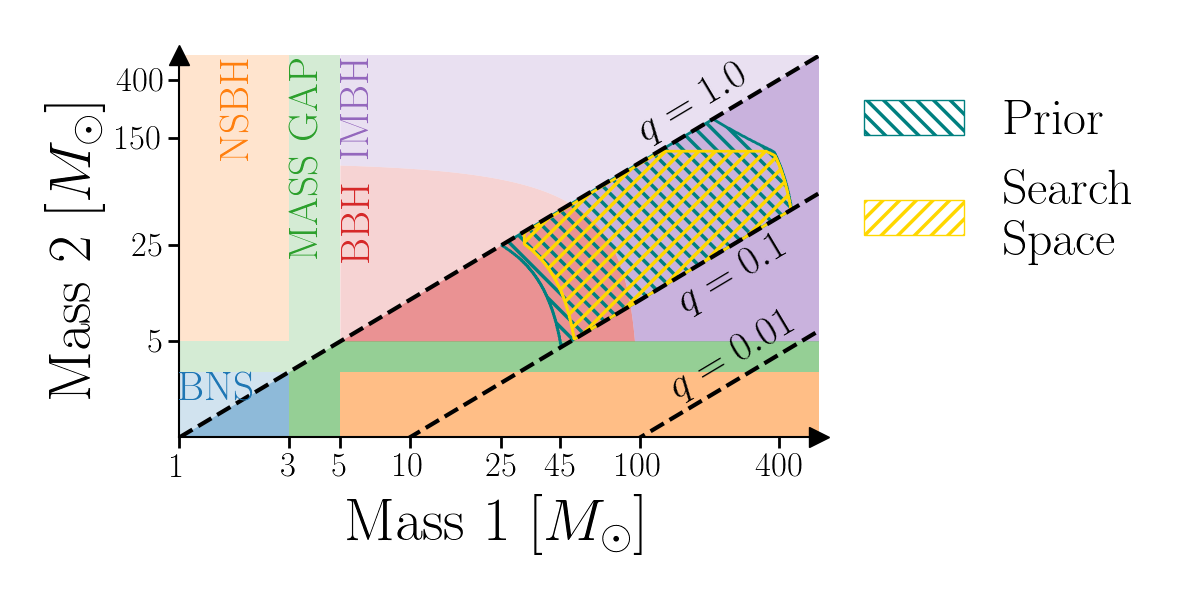
\includegraphics[width=0.75\linewidth]{images/template_bank.png}

}
% time for chunk 14
% 1176955218, Apr 23, 2017, 4:00 UTC
% 1178294418, May 08, 2017, 16:00 UTC
\caption[High-mass BCR search space.]{The template bank (pink) used by \pycbc to search a section of O2 data from $\text{April 23 - May 8, 2017}$. Our search is constrained to the high-mass parameter space enclosed by the dashed line. The candidate, background and simulated triggers detected in this region of the parameter space during this period are plotted in orange, gray and blue respectively.}\label{fig:templateBank}
\end{figure*}


\subsection{Calculating the BCR for triggers}
To evaluate $Z^S$, $Z^G_i$ and $Z^N_i$ and calculate the \bcr Eq.~\ref{eq:bcr} for triggers, we carry out Bayesian inference with \bilby~\cite{bilby, bilby_pipe}, employing \dynesty~\cite{dynesty} as our nested sampler. Nested sampling, an algorithm introduced by~\citet{skilling2004, skilling2006}, provides an estimate of the Bayesian evidence and is often utilized for parameter estimation within the LIGO collaboration~\cite{bilby, bilby_paper, pbilby_paper}.

The most computationally intensive step during Bayesian inference is evaluating the likelihood $\mathcal{L}(d_i|\template)$. To accelerate our analysis, we use a likelihood that explicitly marginalizes over coalescence time, phase at coalescence, and luminosity distance (Eq.~80 from~\citet{intro_to_gw_bayes}).

We set the priors $\pi(\parameters|\mathcal{H}_S)$ and $\pi(\parameters|\mathcal{H}_G)$ to be identical which reflects our ignorance of the distribution of the population properties of signals and signal-like glitches. These priors restrict signals with mass parameters in the ranges presented in Table~\ref{tab:parameters}. The spins are aligned over a uniform range for the dimensionless spin magnitude from $\left[0,1\right]$. The luminosity distance prior assigns probability uniformly in comoving volume, with an upper cutoff of $5\ \text{Gpc}$. The full list of the priors, along with their shapes, limits and boundary conditions are documented in Table~\ref{tab:priors}. 

\begin{table}
    \centering
    \caption{
    Prior settings for the parameters used during our parameter estimation. The definitions of the parameters are documented in \citet{bilby_gwtc}~Table~E1. The trigger time $t_c$ is obtained from the data products of \pycbc's O2 search. \label{tab:priors}} 
    \begin{tabular}{c c c c}
    \hline
    Parameter & Shape & Limits \\
    \hline
          $\mathcal{M}/\msun$           & Uniform & 7--180  \\
          $q$                           & Uniform & 0.1--1  \\
          $M/\msun$                     & Constraint & 50--500  \\
          $d_\mathrm{L}/\mathrm{Mpc}$   & Comoving & 100--5000  \\
          $a_1$, $a_2$                  & Uniform & 0--1  \\
          $\theta_{JN}$                 & Sinusoidal & 0--$\pi$  \\
          $\psi$                        & Uniform & 0--$\pi$  \\
          $\phi$                        & Uniform & 0--$2\pi$  \\
          ra                            & Uniform & 0--$2\pi$  \\
          dec                           & Cosine & 0--$2\pi$  \\
          $t_c/\mathrm{s}$              & Uniform & $t_c\pm0.1$  \\
    \hline
    \end{tabular}
\end{table}

The waveform template we utilize is \imrphenomp, a phenomenological waveform template constructed in the frequency domain that models the in-spiral, merger, and ring-down (IMR) of a compact binary coalescence~\citep{khan2016frequency}. Although there exist gravitational-wave templates such as \seob~\cite{seobnrv4phm} which incorporate more physics, such as information on higher-order modes, we use \imrphenomp as it is computationally inexpensive compared to others.

To generate the PSD, we take 31 neighboring off-source non-overlapping  4-second  segments of time-series data before the analysis data segment $d_i$. To suppress spectral leakage, a Tukey window with a 0.2-second roll-off is applied to each data segment . After this the segments are fast-Fourier transformed and median-averaged to create a PSD~\cite{ligo_psd}. Like other PSD estimation methods, this method adds statistical uncertainties to the PSD~\cite{psd_student_t, chatziioannou2019noise, Biscoveanu:2020:PhRvD}. To marginalize over the statistical uncertainty, we use the median-likelihood presented by~\citet{psd_student_t} as a post-processing step. We find that this post-processing step improves the search efficiency by $49.26\%$ the details of this calculation are presented in the Appendix~\ref{sec:psd-marginalization}.

Finally, we acquire the foreground, background and data in which we inject simulated signals into, from from the gravitational-wave Open Science Center~\cite{GWOSC}. The data we use are the publicly accessible O2 strain data from the Hanford and Livingston detectors, recorded while the detectors are in ``Science Mode''. We obtain the data using \gwpy~\cite{gwpy}. 

\subsection{Assigning \pastro to candidate events}
After the calculating the \bcr for the entire set of high-mass background and simulated triggers, we calculate the background and simulated \bcr probability distributions for each 2-week time-frame of O2 data. These distributions are used to `tune' prior-odd $P^S$ and $P^G$ values as described in Appendix~\ref{apdx:tuning-prior-odds}.

Using the tuned prior odds the \bcr for the candidate events can be calculated. Fig.~\ref{fig:bcrCdf} shows the \bcr distributions for the background triggers, simulated triggers and candidate events. The bulk of the background and simulated trigger distributions are separate but slightly overlap due to some of the simulated signal's being very faint. The separation suggests that the \bcr can successfully distinguish signals from noise or glitches. The vertical lines in Fig.~\ref{fig:bcrCdf} displays the \bcr for gravitational-wave candidate events. On comparing the candidate event \bcr values with the background distribution, we can estimate \pastro values for the candidate events. 

\begin{figure}[!ht]
{\centering 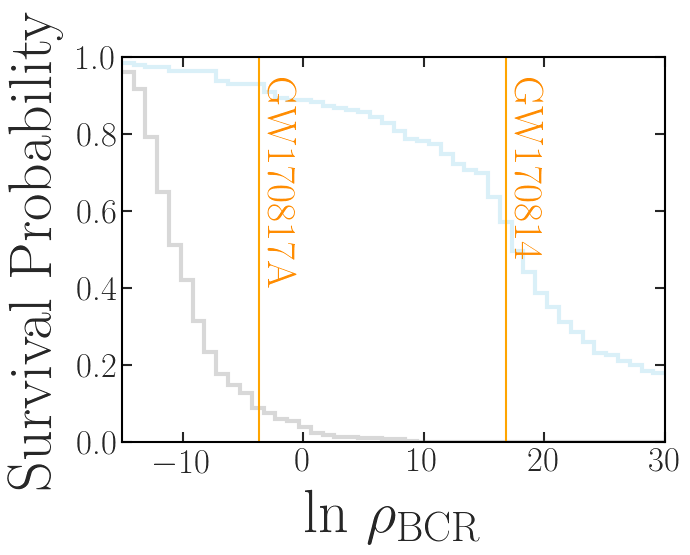
\includegraphics[width=0.85\linewidth]{images/reweighted_bcr_cdf_smaller_legend.png} }
\caption[BCR distribution example]{Histograms represent the survival function (1-CDF) from our high-mass selection of background triggers (gray) and simulated signals (blue) triggers obtained from \pycbc's search of data from $\text{August 13 - 21, 2017}$. Vertical lines mark the $\text{ln}\ \bcr$ of \IAS's GW170817A and \GWTC's GW170814.}\label{fig:bcrCdf}
\end{figure}


\section{\label{sec:Results}Results}

\begin{table*}
\centering
\caption{$\pastrobcr$ table for gravitational wave events and candidates in our search space with $\pastrobcr>0.2$, calculated using Hanford and Livingston observatory data.  Displayed for comparison are significances of events taken from: 
GstLAL \pastroGwtcGstlal~\cite{GWTC1}, 
PyCBC \pastroGwtcPycbc~\cite{GWTC1}, 
IAS \pastroIas~\cite{IAS1, IAS2},  
\pastroPrat~\cite{bayesian_odds}, 
PyCBC `single-search' \pastroSing~\cite{pycbc_single_det}, 
PyCBC OGC-2 \pastroOgcTwo~\cite{pycbc_ogc_2} and
PyCBC OGC-3 \pastroOgcThree~\cite{pycbc_ogc_2}.
The $\tc$ column contains the `GPS' coalescence-times of the gravitational wave events. 
The catalog column displays the first catalog reporting the event on each row (the catalogs labeled IAS-1 and IAS-2 correspond to the candidates published in \citet{IAS1} and \citet{IAS2}).}
\label{tab:results}

\def\arraystretch{1.5} 
\setlength{\tabcolsep}{0.5em}
\begin{NiceTabular}{@{}ll!{\quad}|c|cc!{\quad}c!{\quad}c!{\quad}ccc!{\quad}|c@{}}
\CodeBefore
\rowcolors{2}{white}{gray!10}
\Body


     Event & Catalog & \pastrobcr & \pastroGwtcPycbc & \pastroGwtcGstlal & \pastroIas & \pastroPrat & \pastroSing & \pastroOgcTwo & \pastroOgcThree &          \tc \\
\hline
  GW170104 &  GWTC-1 &        0.97 &              1.00 &               1.00 &             &         1.00 &              &           1.00 &                  & 1167559936.60 \\
  GW170121 &   IAS-1 &        0.83 &                   &                    &        1.00 &         0.53 &              &           1.00 &             1.00 & 1169069154.57 \\
    170209 &       - &        0.32 &                   &                    &             &              &              &                &                  & 1170659643.47 \\
    170222 &       - &        0.58 &                   &                    &             &              &              &                &                  & 1171814476.97 \\
    170302 &   IAS-1 &        0.78 &                   &                    &        0.45 &              &              &                &                  & 1172487817.48 \\
  GW170304 &   IAS-1 &        0.94 &                   &                    &        0.99 &         0.03 &              &           0.70 &             0.70 & 1172680691.36 \\
 GWC170402 &   IAS-2 &        0.60 &                   &                    &        0.68 &         0.00 &              &                &                  & 1175205128.57 \\
  GW170403 &   IAS-1 &        0.54 &                   &                    &        0.56 &         0.27 &              &           0.03 &             0.71 & 1175295989.22 \\
    170421 &       - &        0.27 &                   &                    &             &              &              &                &                  & 1176789158.14 \\
  GW170425 &   IAS-1 &        0.22 &                   &                    &        0.77 &         0.74 &              &           0.21 &             0.41 & 1177134832.18 \\
  GW170608 &  GWTC-1 &        0.99 &              1.00 &               0.92 &             &         1.00 &              &                &                  & 1180922494.50 \\
  GW170727 &   IAS-1 &        0.98 &                   &                    &        0.98 &         0.66 &              &           0.99 &             1.00 & 1185152688.02 \\
  GW170729 &  GWTC-1 &        0.98 &              0.52 &               0.98 &             &         1.00 &              &           1.00 &             0.99 & 1185389807.30 \\
  GW170809 &  GWTC-1 &        0.99 &              1.00 &               0.99 &             &         1.00 &              &           1.00 &             1.00 & 1186302519.75 \\
  GW170814 &  GWTC-1 &        1.00 &              1.00 &               1.00 &             &         1.00 &              &           1.00 &             1.00 & 1186741861.53 \\
 GW170817A &   IAS-2 &        0.92 &                   &                    &        0.86 &         0.02 &              &                &                  & 1186974184.72 \\

\end{NiceTabular}
\end{table*}

We analyze the $60,996$ background, $5,146$ simulated, and $25$ candidate triggers reported by \pycbc's search on the data from LIGO's second observing run, restricting our analysis to the triggers that fall within our mass-space as described in Section~\ref{sec:method}.We also analyze events and candidate events reported by \GWTC and the \IAS group (note: some of these were identified as candidates by the \pycbc search). Table~\ref{tab:results} summaries the \pastrobcr, along with the \pastro of other pipelines for comparison. Although the various pipeline \pastro are not mathematically equivalent, by comparing pipeline \pastro values for a given candidate, we can compare how significant each pipeline deems various candidates. The $P^S$ and $P^G$ values utilized for each time-frame are reported in Appendix~\ref{apdx:alphabeta}.

\subsection{GWTC-1 Events}
All the confirmed gravitational-wave events from binary black hole mergers reported in \GWTC and within our prior space, (specifically GW170104, GW170608, GW170729, GW170809 and GW170814), have $\pastrobcr>0.9$, indicating a high probability of an astrophysical signal. 

In addition to the above confirmed gravitational-wave events from \GWTC, we have also analyzed several candidate events from \GWTC, most of which have low \pastrobcr. For example, consider the candidate event 170412, assigned a $\pastro$ of $0.06$ by \gstlal and has a $\pastrobcr$ of $0.01$. This candidate was reported to be excess power caused due noise appearing non-stationary between 60-200 Hz~\cite{GWTC1}. This candidate acts as an example of how $\pastrobcr$ may be utilized to eliminate candidates originating from terrestrial noise sources.

\subsection{IAS Events}
Our analysis of the high-mass IAS events and candidates in O2 has resulted in three events with disfavored $\pastrobcr<0.5$ (GWC170402, GW170403, GW170425), and four events and one candidate with $\pastrobcr\geq0.5$ (GW170121, 170302, GW170304, GW170727, GW170817A). While GW170727 and GW170817A's \pastrobcr are similar to the \pastro reported from IAS (the differences between the \pastro from \bcr and IAS is $|\Delta \pastro|<0.1$), the remaining candidates have opposing \pastro values (with $|\Delta \pastro| > 0.15$).

GWC170402, detected by \citet{IAS2}, is reported to originate from a binary with non-zero eccentricity~\cite{IAS2}. Hence, we might have received a low \pastrobcr due to our usage of \imrphenomp, a waveform that does not account for eccentricity. Additionally, the search conducted by \citet{IAS2} was a single-detector search. Our ranking statistic relies on the signal to appear coherent, even if just faintly coherent, amongst the various detectors to have a high \pastrobcr. The lack of coherence and the non-eccentric waveform may be the leading factors for a low \pastro. GW170403 and GW170425 which have $\pastrobcr<0.35$ also have low  \pastro reported by \citet{pycbc_ogc_2},  suggesting that these events may have been false alarms.

From the candidates with $\pastrobcr>0.5$, GW170727 and 170302 are of particular interest, with \pastrobcr of $0.92$ and $0.63$. GW170727 was emitted from a black hole binary system with a source frame total mass $\approx 70\ \msun$. In addition to the high \pastrobcr reported by our study, \citet{IAS1} and \citet{pycbc_ogc_2} have also reported high \pastro values of 0.98 and 0.99, making it a viable gravitational-wave event candidate. Similarly, the sub-marginal-candidate 170302 reported by \cite{IAS1} with a \pastro of 0.45 appears to have a higher significance from our analysis, resulting in a \pastrobcr of $0.63$.  


\subsection{New Candidate Events}
Although no clear detections are made with the \bcr, a marginal-candidate 170222 has been discovered with a $\pastrobcr\sim0.5$. This candidate has an SNR$\sim7.7$, low spin magnitudes and source-frame component masses of $({47.16}_{-5.77}^{+8.00}, {35.50}_{-6.35}^{+5.79}) \msun$, making it one of the heavier black-hole mergers from O2 and \GWTC. This candidate may be of interest as one component black hole may lie in the pair-instability mass gap ($55^{+10}_{-10}-148^{+13}_{-12}\msun$)~\cite{Woosley:2021:arXiv, Heger:2002:ApJ}. More details on the candidate are presented in Appendix~\ref{apdx:170222}. The remaining coherent trigger candidates all have $\pastrobcr\ll0.5$ making them unlikely to originate from astrophysical sources. 



\section{\label{sec:Conclusion}Conclusion}

Until 2016, a majority of intermediate-mass black hole candidates were from electromagnetic observations. The dawn of gravitational waves astronomy has provided a new lens to identify and study these massive objects -- from the mergers of heavy black holes' gravitational wave emission. In the future, space-based gravitational wave detectors will uncover black holes in the upper end of the intermediate-mass range. In the present, ground-based gravitational-wave observatories can probe the lower-end of the intermediate-mass range. However, many short-duration terrestrial artifacts that mimic intermediate-mass gravitational-wave signals plague ground-based detectors, making intermediate-mass detection challenging. 

In this paper, we demonstrate that the Bayesian Coherence Odds-Ratio \bcr~\cite{BCR1} can be used as a ranking statistic to provide a measure of significance for gravitational wave signals originating from CBCs with total masses between $55\msun$ and $400\msun$, a range that includes intermediate-mass black holes. To compute the \bcr for candidates, we utilize Bayesian inference to explicitly calculate the probability of data under various hypotheses (the hypotheses that the data contains a coherent signal, just noise, or an incoherent glitch). This Bayesian ranking method takes a step towards building a unified Bayesian framework that provides a search-pipeline agnostic measure of significance for candidates and estimates their parameters, utilizing the same level of physical information incorporated during detected parameter estimation studies. 

In our study, we analyze high-mass candidates detected by \pycbc, the high-mass binary black hole events in O2 reported in \GWTC~\cite{GWTC1} and by the \IAS-team~\cite{IAS1, IAS2}. Using \pastrobcr, we find that the high-mass \GWTC events have high probabilities of originating from an astrophysical source. We also find that some of the \GWTC marginal triggers that have corroborated terrestrial sources (for example, candidate 170412) have low \pastrobcr, indicating this method's ability to discriminate between terrestrial artifacts and astrophysical signals. Our analysis of the high-mass \IAS events demonstrates that GW170121, GW170727, and GW170817A are likely to originate from astrophysical sources, while GWC170402, GW170402, and GW170425  are not. Finally, we do not identify any new gravitational-wave events, but we find a new marginal binary-black hole merger candidate, 170222. 

Although our analysis targets high-mass triggers, this method can be extended to include the entire range of LIGO-detectable gravitational-wave sources. Additionally, to further improve the method's infrastructure, we can use more robust gravitational-wave templates (such as templates that incorporate higher-order modes and orbital precession) and sophisticated glitch models. Future analysis can also incorporate data from all available detectors in a network to increase the sensitivity of \pastrobcr. 


% \greg{can we better constraint their population properties? Do we know how much (if at all) this method outperforms current searches?}

% \avi{Unlike for stellar-mass BBH, there are still alot of uncertainties for IMBH formation scenarios. Hence, upper limits would be challenging to calculate. Additionally, we would require to do more robust simulation studies to see what would fall in/outside our detection threshold, to put constraints on population properties and study the search's sensitivity
% }

%%%%%%---SECTIONS-END---%%%%%%%%%%%%

%%%%%%---ACKNOWLEDGMENTS---%%%%%%%%%%%%
\begin{acknowledgments}

The author gratefully thank the \pycbc team for providing the gravitational-wave foreground, background and simulated triggers from \pycbc's search of O2's data. We also warmly thank Ian Harry and Thomas Dent for answering questions about the \pycbc search's data products.  

We thank Stuart Anderson for assistance with accommodating this analysis which was performed on the California Institute of Technology computing cluster. All analyses (inclusive of test and failed analyses) performed for this study used $~1.3\mathrm{M}$ core-hours, amounting to a carbon footprint of $~167\ \mathrm{t}$ of CO$^2$ (using the US average electricity source emissions of $0.429\ \text{kg/kWh}$~\cite{greenhouse} and $0.3\ \text{kWh}$ for each CPU).

This research has made use of data, software and/or web tools obtained from the Gravitational Wave Open Science Center (https://www.gw-openscience.org), a service of LIGO Laboratory, the LIGO Scientific Collaboration and the Virgo Collaboration. LIGO is funded by the U.S. National Science Foundation. Virgo is funded by the French Centre National de Recherche Scientifique (CNRS), the Italian Istituto Nazionale della Fisica Nucleare (INFN) and the Dutch Nikhef, with contributions by Polish and Hungarian institutes.


\end{acknowledgments}
%%%%%%%%%%%%%%%%%%%%%%%%

\appendix



\section{Bayesian Evidence Evaluation}\label{sec:bayesianEvidEval}
\subsection{Noise Model}
We assume that each detector's noise is Gaussian and stationary over the period being analyzed~\cite{ligo_psd}. In practice, we assume that the noise has a mean of zero that the noise variance $\sigma^2$ is proportional to the noise power spectral density (PSD) \psd of the data. Using the \psd, for each frequency-domain data segment $d_i$ in each of the $i$ detectors in a network of $D$ detectors, we can write 
\begin{equation}
\label{eq:zn}
Z^N_i = \mathcal{N}(d_i|\mu=0,\sigma^2=\psd),
\end{equation}
where $\mathcal{N}$ is a normal distribution. 

\subsection{Coherent Signal Model}
We model coherent signals using a binary black hole waveform template \template, where the vector \parameters contains a point in the 12 dimensional space describing aligned-spin binary-black hole mergers. For the signal to be coherent, \parameters must be consistent in each 4-second data segment $d_i$ for a network of $D$ detectors. Hence, the coherent signal evidence is calculated as
\begin{equation}
\label{eq:zs}
Z^S = \int\limits_{\parameters} \prod\limits^{D}_{i=1} \left[ \mathcal{L}(d_i|\template)\right] \pi(\parameters | \mathcal{H}_S)\  \text{d}\parameters \ ,
\end{equation}
where $\pi(\parameters| \mathcal{H}_S)$ is the prior for the parameters in the coherent signal hypothesis, and $\mathcal{L}(d_i|\template)$ is the likelihood for the coherent signal hypothesis that depends on the gravitational-wave template \template and its parameters \parameters. 

\subsection{Incoherent Glitch Model}
Finally, as glitches are challenging to model and poorly understood, we follow \citet{bci} and utilise a surrogate model for glitches: the glitches are modeled using gravitational-wave templates  \template with uncorrelated  parameters amongst the different detectors such that  $\parameters_i \neq \parameters_j$ for two detectors $i$ and $j$~\cite{bci}.  Modelling glitches with \template captures the worst case scenario: when glitches are identical to gravitational-wave signals (excluding coherent signals). Thus, we can write $Z^G_i$ as 
\begin{equation}
\label{eq:zg}
Z^G_i = \int\limits_{\parameters} \mathcal{L}(d_i|\template)\ \pi(\parameters| \mathcal{H}_G)\  \text{d}\parameters  \ ,
\end{equation}
where $\pi(\theta| \mathcal{H}_G)$ is the prior for the parameters in the incoherent glitch hypothesis. 



\section{Tuning the prior-odds}\label{apdx:tuning-prior-odds}

After calculating the \bcr for a set of background triggers and simulated triggers from as stretch of detector-data (a data chunk), we can compute probability distributions for the background and simulated triggers, $p_b(\bcr)$ and $p_s(\bcr)$. We expect the background trigger and simulated signal \bcr values to favor the incoherent glitch and the coherent signal hypothesis, respectively. Ideally, these distributions representing two unique populations should be distinctly separate and have no overlap in their \bcr values. The prior odds parameters $P^S$ and $P^G$ from Eq.~\ref{eq:bcr} help separate the two distributions. Altering $P^S$ translates the \bcr probability distributions while adjusting $P^G$ spreads the distributions. Although Bayesian hyper-parameter estimation can determine the optimal values for $P^S$ and $P^G$, an easier approach is to adjust the parameters for each data chunk's \bcr distribution. In this study, we tune $P^S$ and $P^G$ to maximally separate the \bcr distributions for the background and simulated triggers. 

To calculate the separation between $p_b(\bcr)$ and $p_s(\bcr)$, we use the Kullback--Leibler divergence (KL divergence) $D_{KL}$, given by
\begin{equation}
    D_{KL}(p_b | p_s) = \sum\limits_{x\in \bcr} p_b(x) \log \left( \frac{p_b(x)}{p_a(x)} \right)  \ .
\end{equation}
The $D_{KL}=0$ when the distributions are identical and increases as the asymmetry between the distributions increases. 

We limit our search for the maximum KL-divergence in the $P^S$ and $P^G$ ranges of $[10^{-10}, 10^0]$. We set our values for $P^S$ and $P^G$ to those which provide the highest KL-divergence and calculate the \bcr for candidate events present in this data chunk. Note that we conduct the analysis in data chunks of a few days rather than an entire data set of a few months as the background may be different at different points of the entire data set.

\section{Marginalizing over PSD statistical uncertainties}\label{sec:psd-marginalization}
To generate the results in Fig.~\ref{fig:bcrCdf}, we applied a post-processing step to marginalize the uncertainty in the PSD. In Fig.~\ref{fig:bcrCdfUnmarginalized}, we show the results if this post-processing step is not applied. Clearly, marginalizing over uncertainty in the PSD yields an improvement in the separation of the noise and signal distributions. Quantitatively, at a threshold $\bcr^T=0$ the post-processing step results in a reduction in the number of background $\bcr > \bcr^T$ from $60.7\%$ to $25.28\%$ in the August 13 - 21, 2017 time-frame of data. For the entirety of O2 PSD marginalization resulted in a $49.26\%$ improvement in search efficiency. 

\begin{figure}[!ht]
{\centering 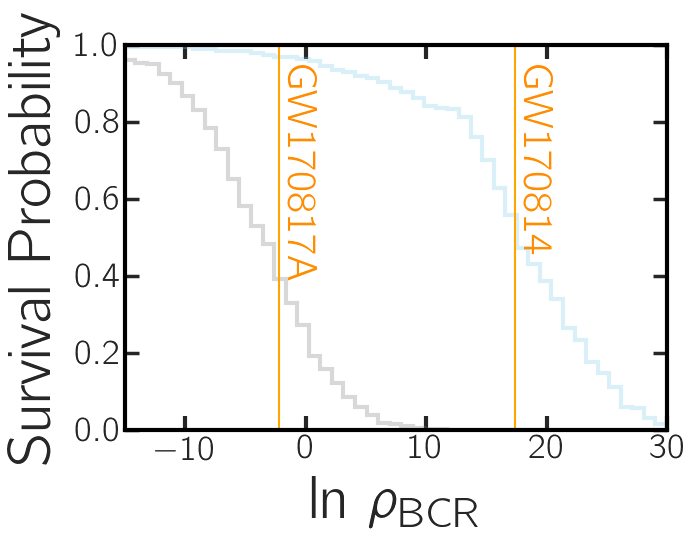
\includegraphics[width=0.85\linewidth]{images/orig_bcr_cdf_smaller_legend.png} }
\caption[BCR distribution example]{This plot is analogous to Fig.~\ref{fig:bcrCdf}, but without using the post-processing step to marginalize over PSD statistical uncertainties. Without the post-processing step, there is a greater overlap between the background (gray) and foreground (blue) survival functions. For more details about this plot, refer to the caption of Fig.~\ref{fig:bcrCdf}.}\label{fig:bcrCdfUnmarginalized}
\end{figure}




\section{Tuned prior odds}\label{apdx:alphabeta}

O2 lasted several months over which the detector's sensitivity varied. Hence, a part of our analysis entailed tuning the prior odds for obtaining a signal and a glitch, $P^S$ and $P^G$, as described in Section~\ref{sec:method}. Table~\ref{tab:priorodds} presents the signal and glitch prior odds utilized for each time-frame of O2 data. 
\begin{table}
\centering
\caption{The prior odds used for each time-frame of data from O2. Each time frame commences at the start date and concludes at the following time-frame's start date.
    }
\label{tab:priorodds}
\def\arraystretch{1.5} 
\setlength{\tabcolsep}{0.5em}
\begin{tabular}{c|cc}

 Start Date &    $\hat{\pi}^S$ &    $\hat{\pi}^G$ \\
\midrule
 2016-11-15 &        - &        - \\
 2016-11-30 &        - &        - \\
 2016-12-23 & 1.00E+00 & 6.25E-01 \\
 2017-01-22 & 1.00E+00 & 2.33E-02 \\
 2017-02-03 & 1.00E-10 & 2.44E-01 \\
 2017-02-12 & 1.76E-08 & 5.96E-02 \\
 2017-02-20 & 6.55E-10 & 2.22E-03 \\
 2017-02-28 & 1.00E-10 & 5.96E-02 \\
 2017-03-10 & 2.56E-10 & 3.91E-01 \\
 2017-03-18 & 1.60E-10 & 1.00E+00 \\
 2017-03-27 & 1.10E-08 & 5.96E-02 \\
 2017-04-04 & 3.73E-02 & 2.33E-02 \\
 2017-04-14 & 1.05E-09 & 2.44E-01 \\
 2017-04-23 & 2.68E-09 & 1.46E-02 \\
 2017-05-08 & 1.00E+00 & 2.44E-01 \\
 2017-06-18 & 6.55E-10 & 3.39E-04 \\
 2017-06-30 & 2.02E-05 & 5.69E-03 \\
 2017-07-15 & 1.05E-09 & 9.54E-02 \\
 2017-07-27 & 1.00E+00 & 2.12E-04 \\
 2017-08-05 & 2.12E-04 & 3.73E-02 \\
 2017-08-13 & 2.68E-09 & 8.69E-04 \\
 2017-08-21 &        - &        - \\

\end{tabular}
\end{table}


Tuning the prior odds can dramatically affect the \pastrobcr. For example, consider Table~\ref{tab:tuningresults}, which reports tuned \pastrobcr and un-tuned \untunedpastrobcr (where $P^S=1$ and $P^G=1$) for various high-mass events and candidates. By tuning the prior odds, the \pastrobcr for some IAS events (for example, GW170403 and GW170817A) can change by more than 0.5, resulting in the promotion/demotion of a candidate's significance.


\begin{table}
\centering
\caption{The BCR p-astro after tuning the prior odds, \pastrobcr, and without tuning the prior odds, \untunedpastrobcr (where $P^S=1$ and $P^G=1$).}
\label{tab:tuningresults}
\def\arraystretch{1.5} 
 \setlength{\tabcolsep}{0.5em}
\begin{tabular}{ll|c c}

     Event &  Catalog & \pastrobcr & \untunedpastrobcr \\
\hline
    161202 &  - &        0.09 &               0.41 \\
  GW170104 &   GWTC-1 &        0.94 &               0.93 \\
  GW170121 &    IAS-1 &        0.76 &               0.72 \\
    170206 &  - &        0.11 &               0.52 \\
    170222 &  - &        0.49 &               0.49 \\
    170302 &    IAS-1 &        0.64 &               0.54 \\
  GW170304 &    IAS-1 &        0.83 &               0.81 \\
 GWC170402 &    IAS-2 &        0.38 &               0.01 \\
  GW170403 &    IAS-1 &        0.33 &               0.89 \\
  GW170425 &    IAS-1 &        0.10 &               0.22 \\
  GW170608 &   GWTC-1 &        0.95 &               0.95 \\
  GW170727 &    IAS-1 &        0.92 &               0.96 \\
  GW170729 &   GWTC-1 &        0.96 &               0.94 \\
  GW170809 &   GWTC-1 &        0.98 &               0.99 \\
  GW170814 &   GWTC-1 &        1.00 &               1.00 \\
 GW170817A &    IAS-2 &        0.83 &               0.36 \\

\end{tabular}
\end{table}



\section{A closer look at 170222}\label{apdx:170222}
PyCBC found the candidate 170222 with $\mathcal{M}_c=49.46$ and $q=0.68$, values that fall within our uncertainty limits. Some of the posteriors that were produced as a by-product of our \bcr calculation can be viewed in Fig.~\ref{fig:170222}.

\begin{figure*}
    \centering
    \begin{subfigure}
        \centering
        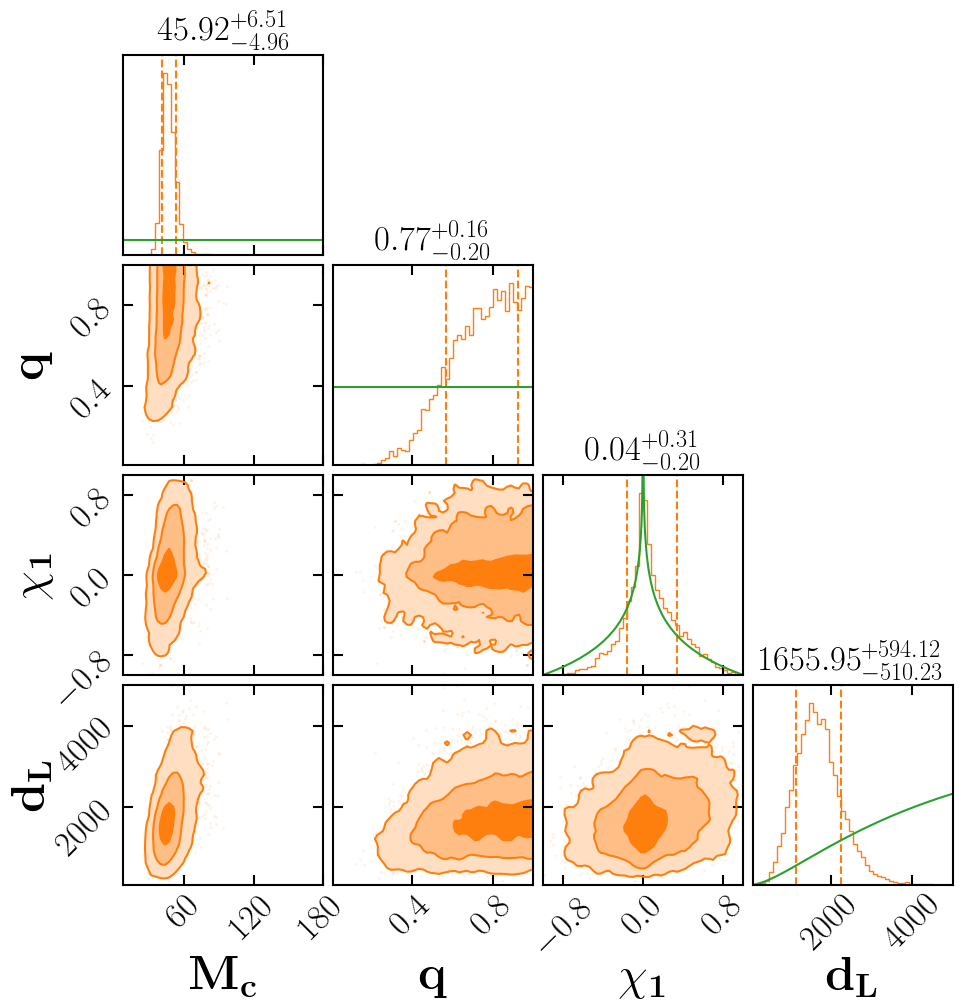
\includegraphics[width=0.45\linewidth]{170222_prior_posterior.png}
    \end{subfigure}
    ~ 
    \begin{subfigure}
        \centering
        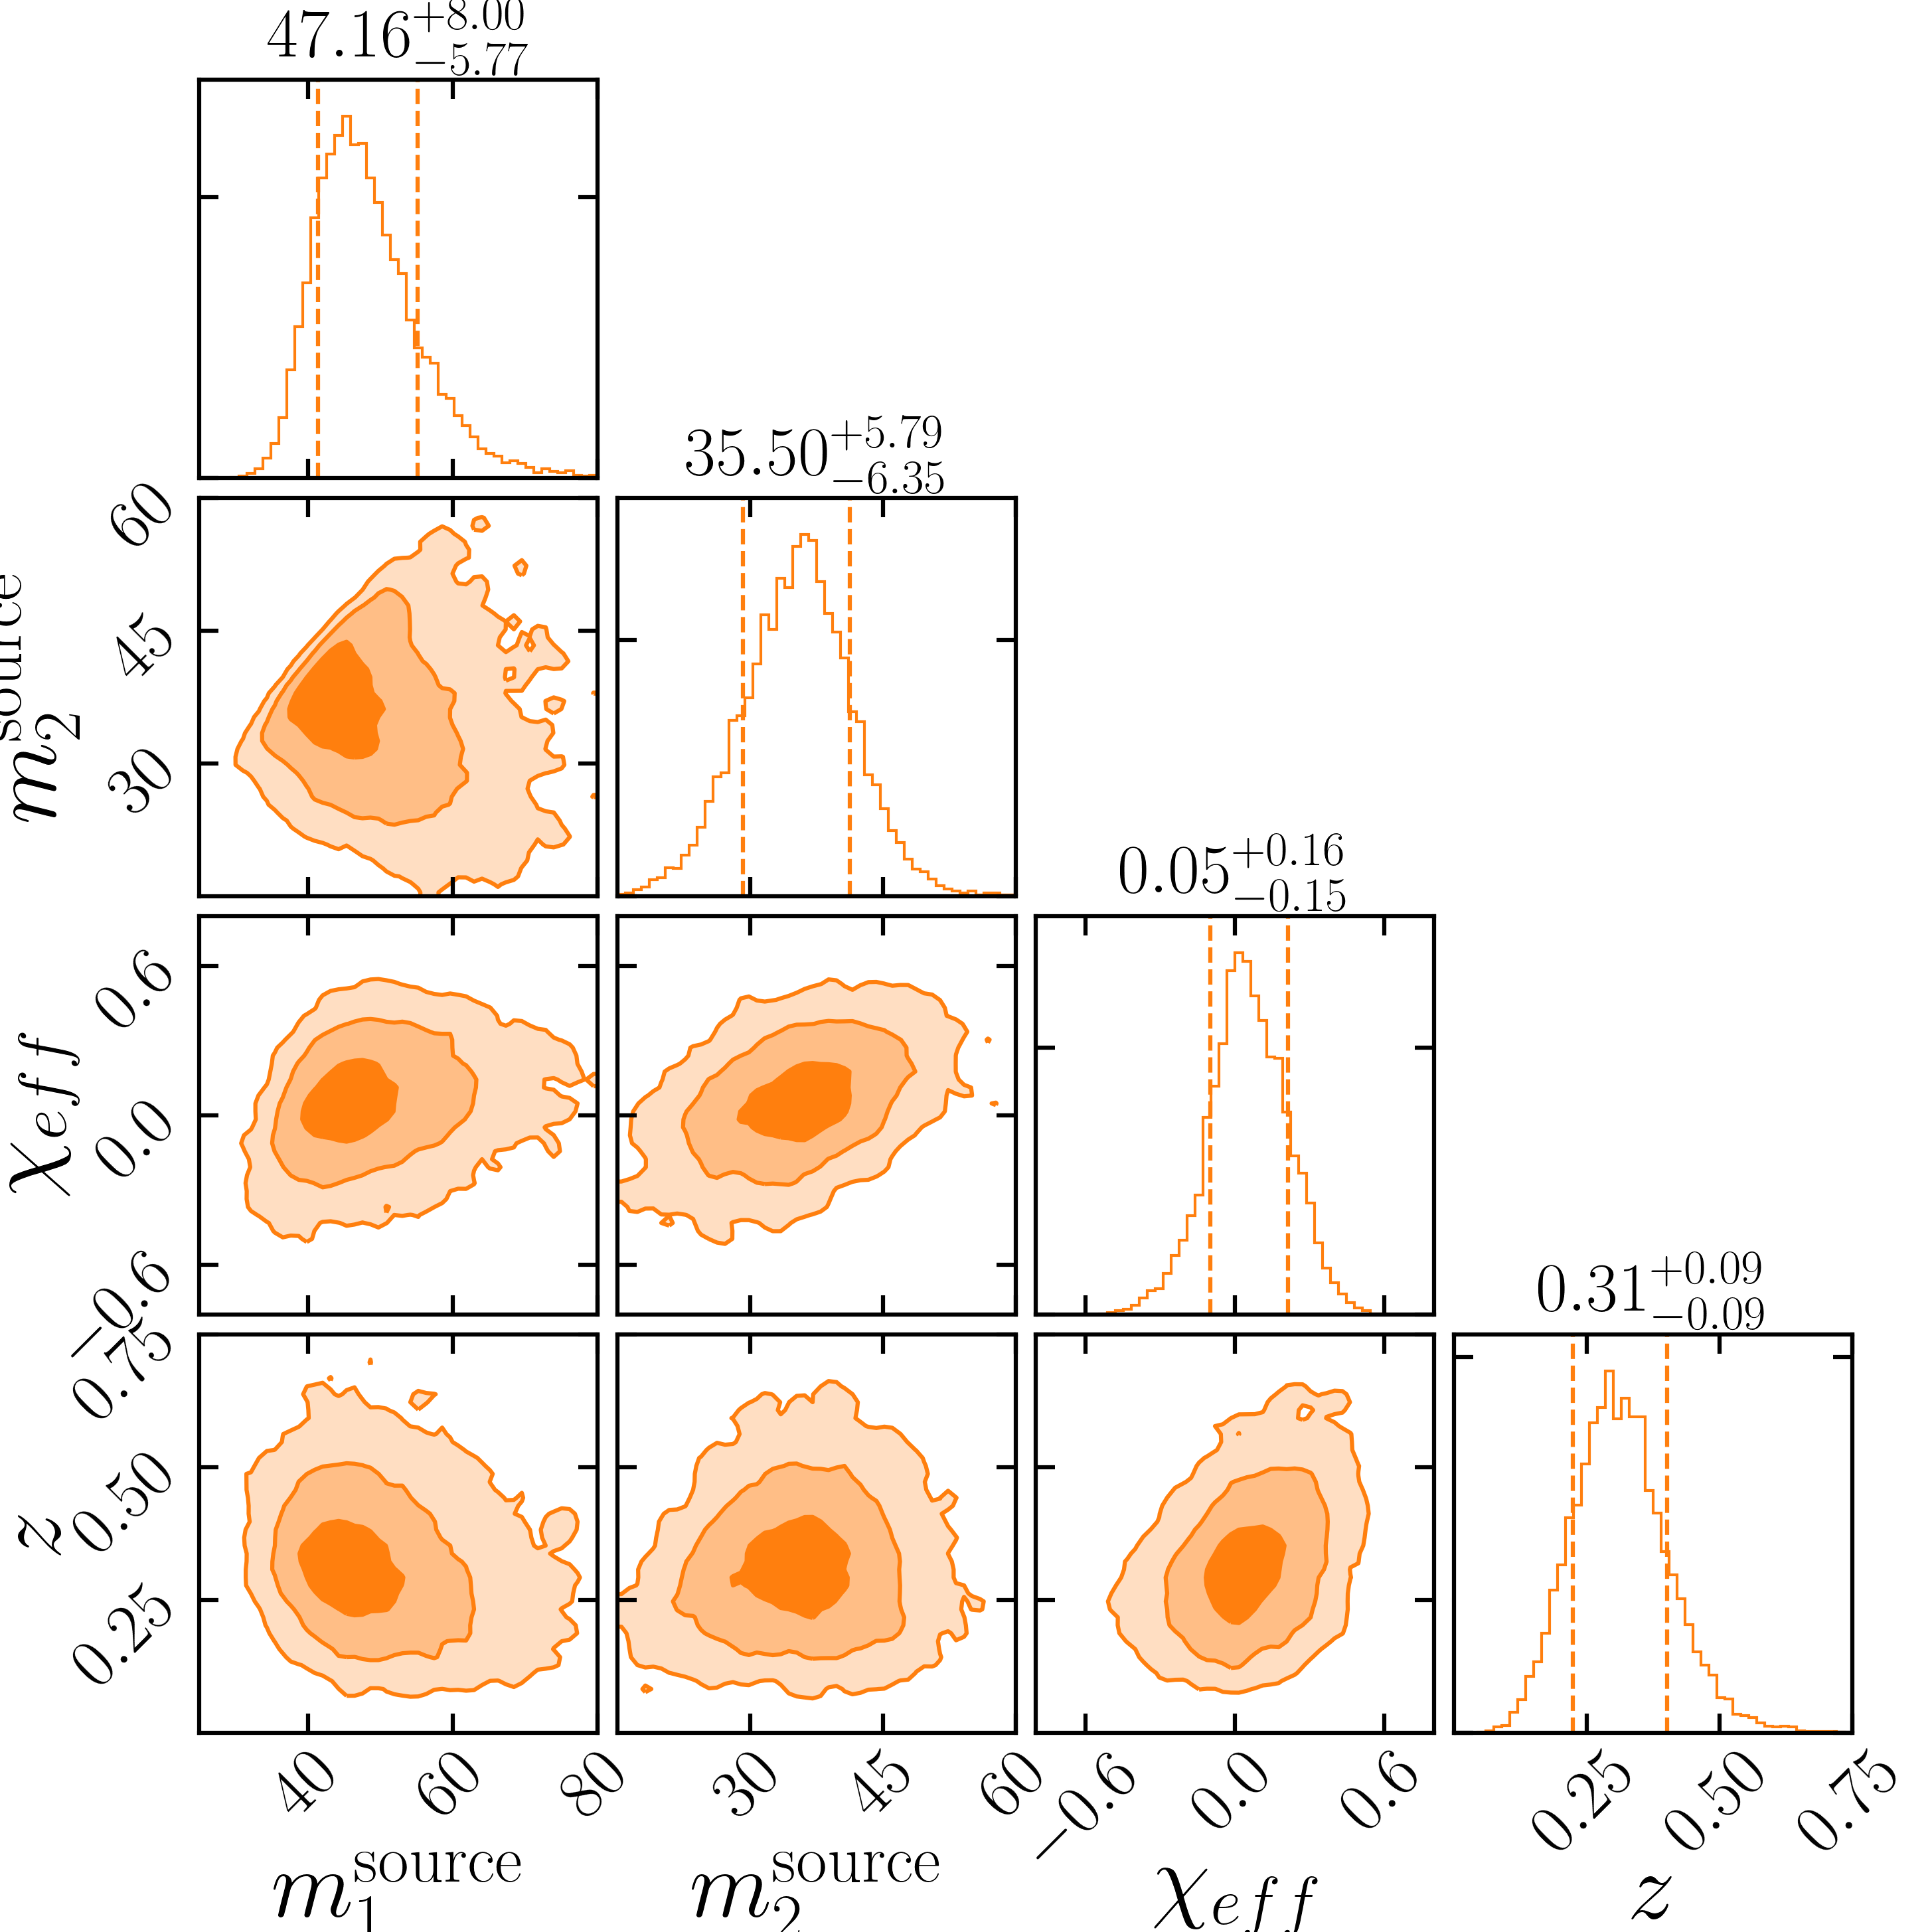
\includegraphics[width=0.45\linewidth]{170222_source_posterior.png}
    \end{subfigure}
    \caption{Posterior distributions for some parameters of 170222. 
    Left: Posterior probability distributions for 4 of the 11 search parameters. Sections of the prior probability density functions used for analysis are displayed in green in one-dimensional marginal distributions plots.
    Right: Posterior probability distributions for some inferred parameters. \avi{Should i plot prior-samples on the right? }
    \label{fig:170222}}
\end{figure*}



% \section{EXTRA INTRO MATERIAL}

% Given the existence of supermassive black holes detected in the early universe, it is likely for intermediate-mass black holes to have also existed~\cite{Banados:2018:Natur, Askar et al  2020,}. However, we only have a handful of promising candidates~\cite{Greene:2004:ApJ, Graham:2013:ApJ, Mezcua:2017:IJMPD, Koliopanos:2017:mbhe, Lin:2020:ApJL, Greene:2020:ARA&A}, and two confirmed intermediate-mass black holes, (i) the $142^{+28}_{-16}\ \msun$ remnant observed from the gravitational wave event GW190521~\cite{Abbott:2020:PhRvL}, and the $5.5^{+1.7}_{-0.9}\times10^{4}\ \msun$ black hole identified from gravitational lensing in the light curve of GRB950830~\cite{paynter_evidence_2021}. The concrete discovery of more intermediate-mass black holes will bridge the observational gap and illuminate our understanding of galaxy and supermassive black hole formation. Additionally, a catalog of observed intermediate-mass black holes can act as probes to their formation environments, such as in the accretion disks of active galactic nuclei~\cite{}, the centers of dense stellar clusters~\cite{}, and even Population-III stars~\cite{}. 

% However, measuring the mass of black holes can be challenging. Several observational techniques to identify intermediate mass black holes

% It is possible to measure the mass of nearby supermassive black holes by directly observing the dynamic motion of stars nearby the supermassive black hole (such as Sgr A$^*$~). However, this dynamic measurement method is challenging to utilize for  intermediate-mass black holes as their sphere of influence is too small to resolve motions~\cite{}. Additionally, dynamic-measurements that have alluded to  intermediate-mass candidates, e.g. the candidate at the center of the globular cluster 47 Tucanae~\cite{kiziltan2017}, can also be attributed to simpler models without a central intermediate-mass black hole~\cite{freire 2017}. }}

% \rs{\sout{In a similar vein, although the M-$\sigma$ and M-L relations (relations between the spheroidal bulge of a galaxy's velocity dispersion $\sigma$,  luminosity L, and its central black hole's mass M) can estimate the mass of supermassive black holes~\cite{Ferrarese & Merritt 2000 and Gebhardt et al. 2000}, they cannot accurately estimate the intermediate-masses. The M-$\sigma$ and M-L relations are not calibrated for low-mass galaxies that might host an central intermediate-mass black hole~\cite{J. E. Greene and L. C. Ho The Mass Function of Active Black Holes in the Local Universe, E. C. Moran, K. Shahinyan, H. R. Sugarman, D. O. Vélez and M. Eracleous Black Holes At the Centers of Nearby Dwarf Galaxies}. Table 2 of~\citet{mercuza} displays a list of intermediate-mass candidates found with these relations. }}

% \rs{\sout{Another method to estimate large black hole masses is with reverberation mapping, which estimates black hole virial masses by studying their nearby gasses' velocities~\cite{reverberation mapping}. Reverberation mapping has shown to estimate both supermassive black hole and intermediate-mass black hole virial masses successfully. However, this method fails to measure the systematic uncertainties on the lower-end of the intermediate-mass spectrum~\cite{}. Additionally, cloud-variability and the possibility of anisotropic emission deride the credibility of intermediate-mass candidates found with reverberation mapping~\cite{}. }}

% The most promising intermediate-mass candidates found with electromagnetic-spectra are Ultra-Luminous X-ray sources with luminosities $> 10^{39} \text{erg s}^{-1}$ (e.g. HLX-X1)~\cite{}. \rs{\sout{While stellar mass black holes are too small to generate such luminosities with Eddington accretion, intermediate mass black holes can accrete at rates large enough to account for the high luminosities~\cite{}. However, some argue that some stellar mass black holes may exceed the Eddington limit~\cite{}, and others argue that the X-ray emission might be from a collimated jet leading to an inaccurate mass calculation~\cite{}.}}


\bibliography{high_mass_bib}% Produces the bibliography via BibTeX.

\end{document}
%
% ****** End of file apssamp.tex ******
